%! alt Triangle ABC with BC = 11 along the bottom, CA = 13 and AB = 20, and A up to the right of C. D on BC has BD = 2 and DC = 9, E on CA has CE = 11, and F on AB has AF = 9. Dashed segments join each of D, E and F to the opposite vertex. Triangle ABD is shaded in the accent tint and triangle ACD in grey: they share AD, and AB + BD = AC + CD = 22, half the perimeter. The area of ABC is 66.
%! after_paragraph 1
%! scale 1/2
% The shared preamble of every Cevian figure. pipeline/figures turns these colours into theme-aware paint,
% and refuses any other colour, so draw only with them:
%   figink (lines and labels), figaux (construction lines), figaccent (the object the argument turns on),
%   figtint and figaccenttint (light fills).
\documentclass[border=1.5pt]{standalone}
\usepackage{tkz-euclide}
\definecolor{figink}{RGB}{0,0,0}
\definecolor{figaux}{RGB}{85,85,85}
\definecolor{figaccent}{RGB}{192,57,43}
\definecolor{figtint}{RGB}{221,221,221}
\definecolor{figaccenttint}{RGB}{245,213,208}
% tkz-euclide's defaults draw circles, compasses and marks in 50% grey and fill points with a tint.
\makeatletter
\def\tkz@otherlinecolor{figink}
\def\tkz@euc@circlecolor{figink}
\def\tkz@euc@compasscolor{figink}
\def\tkz@euc@mkcolor{figink}
\def\tkz@mk@fill{figink}
\def\tkz@euc@pointfillcolor{figink}
\makeatother
\tkzSetUpLine[color=figink,line width=.7pt]
\tkzSetUpArc[color=figink,line width=.7pt]
\tkzSetUpCompass[color=figink,line width=.5pt]
\tkzSetUpPoint[color=figink,fill=figink,size=3.1pt]
\tikzset{
  every picture/.style={line cap=round,line join=round,color=figink},
  circle style/.append style={color=figink,line width=.7pt},
  aux/.style={color=figaux,line width=.45pt,dash pattern=on 2.6pt off 2pt},
  key/.style={color=figaccent,line width=1pt},
  mk/.style={color=figink,line width=.5pt},
  lbl/.style={color=figink,inner sep=2.2pt},
  len/.style={color=figink,inner sep=1.5pt,font=\small},
}

\begin{document}
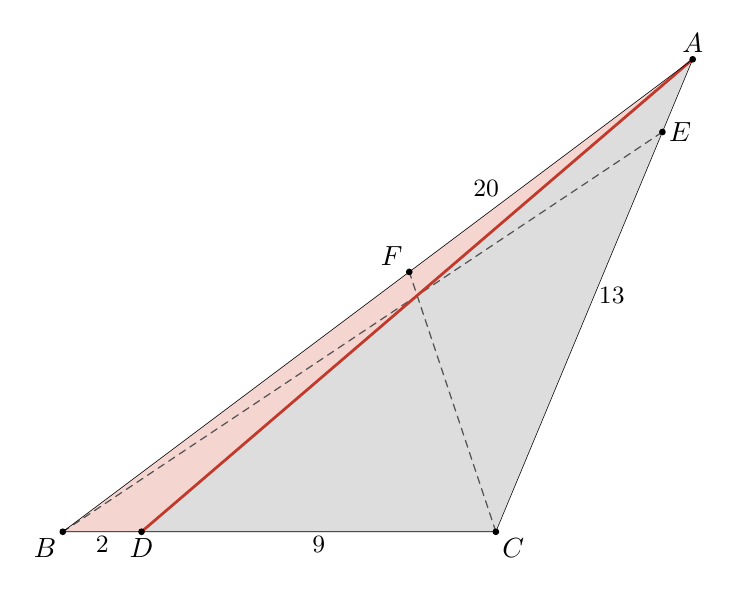
\begin{tikzpicture}
\tkzDefPoint(0.0,0.0){B} %! B = (0, 0)
\tkzDefPoint(5.5000000,0.0){C} %! C = (11, 0)
\tkzDefPoint(8.0000000,6.0000000){A} %! A = (16, 12)
\tkzDefPoint(1.0000000,0.0){D} %! D = (2, 0)
\tkzDefPoint(7.6153846,5.0769231){E} %! E = lerp(C, A, 11/13)
\tkzDefPoint(4.4000000,3.3000000){F} %! F = lerp(A, B, 9/20)
%! fact dist(B, C) == 11
%! fact dist(C, A) == 13
%! fact dist(A, B) == 20
%! fact dist(B, D) == 2
%! fact dist(D, C) == 9
%! fact dist(C, E) == 11
%! fact dist(A, F) == 9
%! fact on_segment(D, B, C)
%! fact on_segment(E, C, A)
%! fact on_segment(F, A, B)
%! fact dist(A, B) + dist(B, D) == 22
%! fact dist(A, C) + dist(C, D) == 22
%! fact dist(B, C) + dist(C, E) == 22
%! fact dist(B, A) + dist(A, E) == 22
%! fact dist(C, A) + dist(A, F) == 22
%! fact dist(C, B) + dist(B, F) == 22
%! fact area(A, B, C) == 66
\tkzFillPolygon[color=figaccenttint](A,B,D)
\tkzFillPolygon[color=figtint](A,D,C)
\tkzDrawSegment[aux](B,E)
\tkzDrawSegment[aux](C,F)
\tkzDrawSegment[key](A,D)
\tkzDrawPolygon(A,B,C)
\tkzDrawPoints(A,B,C,D,E,F)
\tkzLabelPoint[above,lbl](A){$A$}
\tkzLabelPoint[below left,lbl](B){$B$}
\tkzLabelPoint[below right,lbl](C){$C$}
\tkzLabelPoint[below,lbl](D){$D$}
\tkzLabelPoint[right,lbl](E){$E$}
\tkzLabelPoint[above left,lbl](F){$F$}
\tkzLabelSegment[below,pos=.5,len](B,D){$2$}
\tkzLabelSegment[below,pos=.5,len](D,C){$9$}
\tkzLabelSegment[right,pos=.5,len](C,A){$13$}
\tkzLabelSegment[above left,pos=.3,len](A,B){$20$}
\end{tikzpicture}
\end{document}
